\chapter{Classificazione dei Segnali}
Piglio un segnale analogico posso convertirlo in un segnale numerico (digitale) con un \textbf{trasduttore} (convertitore A/D).

Un segnale periodico si ripete ogni T secondi.
  
\begin{center}
  La \textbf{sinusoide} ha:
  \begin{tabular}{ll}
    \textbf{Ampiezza} & A \\
    \textbf{Pulsazione} & $\frac{2\pi}{T}$ \\
    \textbf{Fase} & $\phi$\\
    \textbf{Frequenza} & $f_0 = \frac{1}{T} $\\
  \end{tabular}

  $Acos(\frac{2\pi }{T} + \phi )$
\end{center}

Espressione generale segnale periodico: $x(t) = \sum ^\infty _{k = -\infty} w(t-kT)$
\begin{center}
  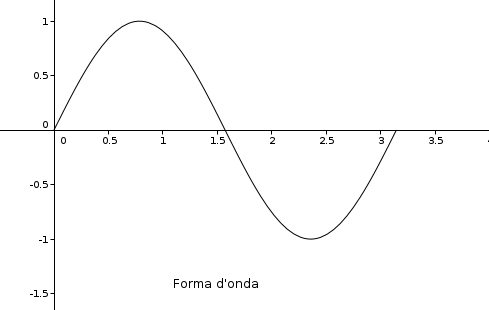
\includegraphics[scale=0.5]{Chapters/Img/c01_01.png}
\end{center}

Un segnale \'e \textbf{deterministico} se il valore \'e univocamente determinato fissate le sue variabili di dominio (tempo o spazio).
La sinusoide \'e deterministica dato che \'e determinabile per ogni valore della variabile di dominio.

Non esiste un orologio elettronico che abbia jitter (a priori non posso sapere il periodo)

Per il semplice fatto che un conduttore esiste sopra gli 0K, implica la presenza di correnti termiche di livello quantistico (rumore termico).

Per rappresentare una funzione complessa uso modulo e fase (due eq. reali).

Formula di Eulero:
$e^{j\theta} = cos \theta + jsin\theta \implies cos\theta = \frac{e^{j\theta} + e^{-j\theta}}{2},\ sin\theta = \frac{e^{j\theta} - e^{-j\theta}}{2j}$

Posso rappresentare un numero complesso con coordinate polari: $x + iy = r cos \theta + jrsin \theta = re^{j\theta }$
con r la distanza dal polo (origine) 

Corrente alternata (modulo, frequenza e fase); ho un fasore che ruota attorno ad un asse reale.


